% Vietnamese translation for OI Public Library
% Source-PDF: IOI中国国家候选队论文/2000/杨江明论文.pdf
\documentclass[11pt]{article}
\usepackage{tikz}
\usepackage{oipl-vn}

\title{Bàn về ứng dụng chiến lược toán học trong các bài toán tin học}
\author{Yang Jiangming}
\date{}

\begin{document}
\maketitle

\origtitle{On the application of mathematical strategies in informatics problems}
\sourcepath{IOI China candidate team papers / 2000 / Yang Jiangming.pdf}

\paragraph{Từ khóa.}
Chiến lược; khả năng mở rộng; hiệu suất; bài toán nguyên.

\section*{Tóm tắt}

Bài viết này nghiên cứu các chiến lược toán học, một nội dung rất quan trọng
trong thi tin học nhưng thường bị xem nhẹ. Thông qua việc phân tích cách dùng
tư tưởng phương trình, tư tưởng bất đẳng thức và phương pháp xây dựng trong
các bài toán cụ thể, bài viết so sánh ưu khuyết điểm của chúng với những
chiến lược khác, đồng thời trình bày tương đối chi tiết hiệu suất, phạm vi áp
dụng và khả năng mở rộng của chiến lược toán học. Bài viết cũng tổng kết lý
do đưa chiến lược toán học vào các bài toán tin học, từ đó gợi ra cách dùng
chiến lược toán học trong quá trình giải bài nói chung, và nhìn về triển
vọng ứng dụng của nó trong các kỳ thi tin học sau này. Các ví dụ trong bài
đều lấy từ đề thi tin học các cấp trong những năm gần đây; với một số bài,
bài viết nêu cách giải bằng chiến lược toán học hiệu quả hơn thuật toán
chuẩn, nên có ý nghĩa thực tiễn rõ rệt.

\tableofcontents

\section{Toán học và chiến lược}

Toán học là khoa học nghiên cứu hình thức không gian và quan hệ số lượng của
thế giới hiện thực; nó là công cụ mạnh để xử lý các vấn đề khách quan và giữ
vai trò nền tảng trong hầu như mọi ngành khoa học tự nhiên.

Chiến lược là phương pháp được dùng để giải quyết vấn đề. Nó bao gồm các
phương pháp giải nhiều loại vấn đề và nhiều mặt của cùng một vấn đề. Chiến
lược được bàn trong bài này là những phương pháp hữu hiệu được dùng khi lập
trình trên máy tính để giải bài, tức là chiến lược lập trình.

Những chiến lược thường gặp khi viết chương trình giải bài gồm: chiến lược
toán học, hay chiến lược quy luật; chia để trị; tham lam; liệt kê, bao gồm
tìm kiếm; v.v.

Khi đánh giá một chiến lược tốt hay xấu, ta thường xét ba phương diện.

\begin{enumerate}
  \item \term{Hiệu suất.} Đây chính là độ phức tạp thuật toán. Trong thi đấu,
  khi xét độ phức tạp của chương trình, người ta thường xét độ phức tạp thời
  gian. Dĩ nhiên, độ phức tạp thời gian và độ phức tạp không gian ràng buộc
  lẫn nhau.

  \item \term{Phạm vi áp dụng.} Nghĩa là chiến lược ấy có thể giải những loại
  bài nào; đây là sự khái quát tổng thể về những bài mà ``mọi'' thuật toán
  thuộc chiến lược đó có thể giải.

  \item \term{Khả năng mở rộng.} Với thuật toán được xây dựng cho một bài cụ
  thể, liệu nó có thể tiếp tục dùng cho bài khác hay không. Nếu một thuật
  toán có thể dùng trên nhiều bài, ta nói thuật toán ấy có khả năng mở rộng
  lớn.
\end{enumerate}

Với các chiến lược toán học được nghiên cứu dưới đây, ta đều so sánh chúng
với các chiến lược khác từ ba phương diện này.

Theo nghĩa rộng, chiến lược toán học bao gồm chiến lược dùng lý thuyết đồ thị,
chiến lược quy hoạch động, và chiến lược dùng các công cụ toán sơ cấp. Trong
những năm gần đây, lý thuyết đồ thị và quy hoạch động xuất hiện rất thường
xuyên trong các kỳ thi; ngược lại, những phương tiện trong toán sơ cấp như tư
tưởng phương trình và tư tưởng bất đẳng thức, vốn dùng để đơn giản hóa đề bài
và giải quyết vấn đề, lại chưa được coi trọng đúng mức. Thực ra, sử dụng
những phương tiện cơ bản ấy là tiền đề không thể thiếu để đơn giản hóa điều
kiện đã biết của đề và xây dựng một mô hình toán học tốt. Đôi khi chúng còn
đem lại kết quả bất ngờ.

Chiến lược toán học trong bài này được hiểu theo nghĩa hẹp: chiến lược sử
dụng các công cụ toán sơ cấp. Thông qua phân tích một số bài thi tin học
trong những năm gần đây, bài viết so sánh sự khác biệt rất lớn về hiệu suất
giữa việc dùng chiến lược toán học để giải hoặc đơn giản hóa bài toán với
việc trực tiếp dùng các chiến lược thông thường. Từ đó, bài viết cho thấy
tiềm năng lớn và ưu thế giải bài của chiến lược toán học trong thi tin học,
đồng thời thử tổng kết các bước nên có khi giải một bài toán nói chung.

\section{Ứng dụng chiến lược toán học trong bài toán tin học}

Hãy nhìn xem con người giải các vấn đề cụ thể như thế nào. Bản thân con người
không có hệ thống tính toán nhanh, cũng không có hệ thống lưu trữ dung lượng
lớn; điều ta dựa vào khi giải bài là suy luận logic mà ta thành thạo, cùng
các công cụ toán học mạnh. Ta có lý thuyết phương trình, tư tưởng bất đẳng
thức, v.v.; đó lại chính là điều máy tính còn thiếu. Vì vậy ta thử làm cho
máy tính cũng có các ưu điểm ấy. Chiến lược tham lam, thuật toán \(A^*\), và
nhiều kỹ thuật khác thực chất đều là những thử nghiệm có ích theo hướng đó:
dùng cách suy nghĩ của con người để thực hiện một số lựa chọn. Còn chiến lược
toán học đang được bàn ở đây chính là việc dùng trực tiếp các công cụ toán
học ấy. Xem Phụ lục~\ref{app:notes}.

Việc dùng chiến lược toán học trong tin học gồm hai mặt: đơn giản hóa đề bài
và trực tiếp giải bài.

Dùng chiến lược toán học để đơn giản hóa đề bài là một bước quan trọng không
thể thiếu khi giải bài, đồng thời là phương pháp cơ bản để phân tích đề. Bằng
cách dùng chiến lược toán học để đơn giản hóa đề bài, ta phát hiện các điều
kiện ẩn trong đề, tìm thêm nhiều điều kiện ``đã biết'', qua đó đặt nền móng
tốt cho việc xây dựng mô hình toán học. Còn nếu dùng chiến lược toán học để
giải trực tiếp, hiệu suất của nó càng là điều các thuật toán thông thường
khó đạt tới.

Dưới đây, ta lần lượt phân tích ứng dụng của chiến lược toán học qua ba mặt:
phương trình, bất đẳng thức và phương pháp xây dựng.

\subsection{Tư tưởng phương trình trong chiến lược toán học}

\begin{center}
\textit{Con đường để đơn giản hóa và giải quyết đề bài}
\end{center}

Phương trình được xây dựng trên cơ sở đề bài, là sự trừu tượng hóa và tổng
kết các điều kiện. Đối với những điều kiện khác nhau của cùng một bài toán,
phương trình có tính áp dụng phổ quát. Vì vậy, phương trình bù đắp nhược điểm
của chiến lược liệt kê, bao gồm tìm kiếm: phải thử mọi trường hợp mới rút ra
kết luận.

Phương trình là một phương tiện khá quan trọng trong chiến lược toán học. Nói
chung, khi dùng phương trình để giải bài, ta thường giải hệ phương trình đại
số tuyến tính \(n\) ẩn, một việc tương đối phù hợp với chương trình; do đó
liên quan đến phương pháp khử Gauss để giải loại hệ phương trình này.

Sau đây nhắc lại cách dùng khử Gauss để giải hệ phương trình tuyến tính. Dạng
tổng quát của một hệ tuyến tính \(n\) ẩn bậc \(n\) là
\[
\begin{aligned}
  a_{11}x_1+a_{12}x_2+\cdots+a_{1n}x_n&=b_1,\\
  a_{21}x_1+a_{22}x_2+\cdots+a_{2n}x_n&=b_2,\\
  &\vdots\\
  a_{n1}x_1+a_{n2}x_2+\cdots+a_{nn}x_n&=b_n.
\end{aligned}
\]

Trong đại số, hệ phương trình thường được giải bằng khử biến. Trước hết nhân
hàng thứ nhất với một hằng số rồi cộng với các hàng khác để khử hạng tử chứa
\(x_1\) ở các hàng còn lại, tức làm cho \(a_{21},a_{31},\ldots,a_{n1}\) bằng
0. Sau đó dùng hàng thứ hai mới nhân với một hằng số rồi cộng với các hàng từ
thứ ba đến thứ \(n\), để khử hạng tử chứa \(x_2\) ở các hàng này. Tiếp tục như
vậy, cuối cùng dùng hàng thứ \(n-1\) mới để khử hạng tử chứa \(x_{n-1}\) ở
hàng thứ \(n\). Ta thu được hệ tam giác:
\[
\begin{aligned}
  a_{11}x_1+a_{12}x_2+a_{13}x_3+\cdots+a_{1n}x_n&=b_1,\\
  a'_{22}x_2+a'_{23}x_3+\cdots+a'_{2n}x_n&=b'_2,\\
  a'_{33}x_3+\cdots+a'_{3n}x_n&=b'_3,\\
  &\vdots\\
  a'_{nn}x_n&=b'_n.
\end{aligned}
\]

Quá trình khử tiến và thế ngược có thể tóm tắt bằng sơ đồ sau. Từ phương
trình cuối cùng có thể trực tiếp tính \(x_n=b'_n/a'_{nn}\), rồi lần lượt thế
ngược để tìm \(x_{n-1},x_{n-2},\ldots,x_1\).

\begin{center}
\begin{tikzpicture}[
  box/.style={draw,rounded corners=1pt,align=center,text width=2.55cm,
    minimum height=0.78cm,font=\small},
  edge/.style={->,thick}
]
  \node[box] (input) at (0,0) {Hệ tuyến tính\\\(n\) phương trình};
  \node[box] (pivot) at (3.25,0) {Với \(i=1,\ldots,n-1\)\\chọn hàng trụ};
  \node[box] (check) at (6.5,0) {Nếu \(a_{ii}=0\)\\đổi hàng};
  \node[box] (elim) at (9.75,0) {Khử \(x_i\)\\ở các hàng dưới};
  \node[box] (tri) at (6.5,-1.75) {Sau mọi cột\\thu hệ tam giác};
  \node[box] (back) at (3.25,-1.75) {Thế ngược\\từ \(x_n\) về \(x_1\)};
  \node[box] (fail) at (9.75,-1.75) {Không có hàng trụ:\\vô nghiệm hoặc vô số nghiệm};

  \draw[edge] (input) -- (pivot);
  \draw[edge] (pivot) -- (check);
  \draw[edge] (check) -- (elim);
  \draw[edge] (elim) -- (tri);
  \draw[edge] (tri) -- (back);
  \draw[edge] (check) -- (fail);
\end{tikzpicture}
\end{center}

Còn phải xét một vấn đề: nếu trong quá trình trên có \(a_{ii}=0\), phép khử
có thể yêu cầu nhân hàng thứ \(i\) với hằng số \(a_{ki}/a_{ii}\), gây vô hạn
và tràn số. Chẳng hạn, để khử hạng tử \(x_1\) ở hàng thứ hai, vốn phải thực
hiện ``phương trình (1) nhân \(a_{21}/a_{11}\) trừ phương trình (2)''; nếu
\(a_{11}=0\), sẽ có lỗi tràn. Do đó cần bảo đảm \(a_{ii}\ne 0\). Nếu xảy ra
\(a_{ii}=0\), ta tìm một hàng \(m\) trong các hàng từ \(i+1\) đến \(n\) sao
cho \(a_{mi}\ne0\), rồi đổi chỗ hàng \(m\) với hàng \(i\). Nếu không tìm được,
hệ phương trình vô nghiệm hoặc có vô số nghiệm.

Theo phương pháp vừa nêu, trước hết khử tiến để thu được hệ tam giác. Sau đó
chuẩn hóa để các \(A_{ii}\) trong hệ tam giác đều bằng 1:
\[
\begin{aligned}
  x_1+a''_{12}x_2+a''_{13}x_3+\cdots+a''_{1n}x_n&=b''_1,\\
  x_2+a''_{23}x_3+\cdots+a''_{2n}x_n&=b''_2,\\
  &\vdots\\
  x_{n-1}+a''_{(n-1)n}x_n&=b''_{n-1},\\
  x_n&=b''_n.
\end{aligned}
\]
Khi đó \(x_n=b''_n\), rồi thế ngược để tìm \(x_{n-1},\ldots,x_1\). Trong cài
đặt, để rõ ràng, tốt nhất dùng các chương trình con, mỗi chương trình con
hoàn thành một chức năng.

Kỳ IOI 1999 vừa qua để lại cho ta nhiều điều đáng nghĩ. Ta bắt đầu từ bài
toán chia bài trong IOI 1999.

\subsubsection{Vận dụng tư tưởng phương trình}

\paragraph{Ví dụ 1. Bài toán chia đều quân bài.}
Đây là một trò chơi chia đều quân bài. Có \(N\) cột quân bài, mỗi cột có một
số quân bài, có thể là 0. Các cột được đánh số bằng các số nguyên từ 1 đến
\(N\). Khi di chuyển quân bài, cần chỉ định một cột xác định \(p\) và một số
xác định \(m\). Sau đó chuyển \(m\) quân bài từ cột \(p\) sang mỗi cột kề
với nó. Nếu \(1<p<N\), cột \(p\) có hai cột kề là \(p-1\) và \(p+1\); nếu
\(p=1\), nó chỉ có một cột kề là cột 2; nếu \(p=N\), nó chỉ có một cột kề là
cột \(N-1\).

Chú ý rằng nếu cột \(p\) có hai cột kề, khi thực hiện thao tác trên thì cột
\(p\) phải có ít nhất \(2m\) quân bài; nếu cột \(p\) chỉ có một cột kề, thì
cột \(p\) cần ít nhất \(m\) quân bài.

Mục tiêu của trò chơi là ``chia đều'' mọi cột quân bài, sao cho mỗi cột có
cùng số quân bài, và đạt mục tiêu ấy với số lần di chuyển ít nhất. Nếu có hơn
một cách di chuyển thỏa yêu cầu, chỉ cần đưa ra một cách. Xem
Phụ lục~\ref{app:notes}.

Ta dùng chiến lược toán học để đơn giản hóa đề bài nhằm tìm ý tưởng tốt hơn;
chỉ khi đơn giản hóa được đề bài mới có thể giải tốt hơn. Nhưng thực tế, khi
nhiều người cầm bài này lên, họ đều lúng túng: làm sao mới có thể ``chia
đều''? Thế là các thuật toán đã học bắt đầu va chạm trong đầu.

\begin{quote}
Thí sinh: Tìm kiếm, bạn làm được không?

Tìm kiếm: Ừm, đến 10000 bước đấy; nếu để tôi làm thì e phải chờ khá lâu.

Thí sinh: Quy hoạch động, còn bạn?

Quy hoạch động: Tôi ư? Bài này tôi cũng chịu.
\end{quote}

Làm thế nào? Trước hết, ta phân tích đề bài và phải nhận ra một tầng quan hệ:
các quân bài ở cột \(i\) chỉ có thể chuyển sang hai phía, tức các cột \(i+1\)
và \(i-1\); đồng thời tổng số quân chuyển sang hai phía là bằng nhau, trừ cột
1 và cột \(n\).

Thứ hai, chỉ các cột \(i+1\) và \(i-1\) có thể chuyển quân bài vào cột \(i\),
và số quân chuyển vào cột \(i\) tất yếu bằng một nửa tổng số quân chuyển đi
của hai cột \(i+1\) và \(i-1\). Để bảo đảm chia đều, hiệu giữa tổng số quân
bài cột \(i\) chuyển đi và tổng số quân bài chuyển vào cột \(i\) tất yếu bằng
hiệu số quân bài giữa trạng thái đầu và trạng thái cuối. Trạng thái đầu là
trạng thái ban đầu; trạng thái cuối là trạng thái đều. Vì vậy, với \(N\) cột
quân bài có \(N\) ẩn, chính là tổng số quân bài mỗi cột phải chuyển đi. Ký
hiệu số quân bài cột \(i\) phải chuyển đi là \(M_i\), hiệu giữa trạng thái đầu
và trạng thái cuối của cột \(i\) là \(\Delta_i\). Ta có hệ phương trình:
\[
\begin{array}{rcl@{\qquad}rcl}
M_2-M_1&=&A-C_1=\Delta_1, & M_2-M_1&=&\Delta_1,\\
M_1-2M_2+M_3&=&A-C_2=\Delta_2, & M_3-M_2&=&\Delta_1+\Delta_2,\\
M_2-2M_3+M_4&=&A-C_3=\Delta_3, & M_4-M_3&=&\Delta_1+\Delta_2+\Delta_3,\\
M_3-2M_4+M_5&=&A-C_4=\Delta_4, & &\vdots&\\
\vdots&&\vdots, & &\vdots&\\
M_{n-2}-2M_{n-1}+M_n&=&A-C_{n-1}=\Delta_{n-1},&
M_n-M_{n-1}&=&\Delta_1+\Delta_2+\cdots+\Delta_n,\\
M_n-M_{n-1}&=&A-C_n=\Delta_n.&&&
\end{array}
\]
Vế phải là kết quả sau khi dùng khử Gauss để đơn giản hóa.

Có \(n\) ẩn và \(n-1\) phương trình, nên đây là một hệ bất định. Giả sử
\(M_1=0\), thay vào có thể tìm được một nghiệm
\(\{x_1,x_2,x_3,\ldots,x_n\}\), trong đó \(x_1=0\). Theo tính chất của hệ
phương trình tuyến tính \(n\) ẩn,
\[
  \{x_1+t,x_2+t,x_3+t,\ldots,x_n+t\},
\]
với \(t\) là số nguyên, cũng nhất định là một nghiệm của hệ; thay vào hệ đã
đơn giản hóa là có thể chứng minh.

Đề bài yêu cầu số lần di chuyển nhỏ nhất; dĩ nhiên tổng số quân bài được di
chuyển cũng phải cố gắng nhỏ. Vì \(x_i\ge0\), nếu tìm được một nghiệm trong
đó nghiệm nhỏ nhất bằng 0, thì tổng số quân bài di chuyển ứng với nghiệm ấy
nhất định là nhỏ nhất. Ta rút ra kết luận:
\begin{quote}
Số quân bài mỗi cột cần chuyển đi là xác định, có thể tính được, và có thể
bảo đảm chia đều.
\end{quote}

Khi đã có bảo đảm chia đều, phần còn lại dễ xử lý hơn nhiều. Dùng chiến lược
tham lam, thuật toán ngẫu nhiên hóa, hoặc phối hợp vài thuật toán đều được.
Ngay cả thuật toán tham lam cơ bản nhất cũng đủ xử lý dữ liệu kiểm thử của
IOI 1999.

Thực ra bài này của IOI 1999 nhắc ta rằng toán học rốt cuộc vẫn là nền tảng.
Không có thuật toán nào hoàn toàn tách khỏi toán học; tách khỏi việc phân
tích bản thân đề bài mà chỉ máy móc áp dụng thuật toán là điều không thực tế.
Đây chính là lỗi mà nhiều thí sinh thường mắc.

Ta xét tiếp một bài liên quan.

\paragraph{Ví dụ 2. Bài toán điện trở.}
Trong vật lý, ta thường đau đầu với những mạch điện phức tạp. Để tiện phân
tích, ta cần thay một mạch hỗn hợp gồm các điện trở bằng một điện trở tương
đương. Việc tính điện trở tương đương thường rất rườm rà, vì vậy ta thử dùng
chương trình để hoàn thành công việc này. Chương trình cần tính tổng điện trở
giữa hai điểm trong một mạch hỗn hợp chỉ gồm điện trở. Xem
Phụ lục~\ref{app:notes}.

\paragraph{Mô tả.}
Để tiện trình bày, ta xây dựng mô hình sau để mô tả mạch: mạch được tạo bởi
các nút nối với nhau; nút là giao điểm của dây dẫn. Nếu trên đoạn mạch giữa
hai nút không có nút nào khác, gọi hai nút ấy là hai nút kề nhau. Giữa hai
nút kề nhau chỉ cho phép hai trường hợp:
\begin{enumerate}
  \item giữa chúng là một điện trở đã biết;
  \item giữa chúng là mạch song song thuần gồm \(x\) điện trở đã biết.
\end{enumerate}
Tổng điện trở giữa hai nút kề nhau không bằng 0; nếu bằng 0, hai nút ấy có
thể gộp thành một nút. Không có nút cô lập.

Mô hình này tất nhiên có thể mô tả mọi mạch thuần điện trở. Trên cơ sở đó ta
phân tích bài toán này.

\paragraph{Dữ liệu vào.}
Dòng đầu là số nguyên \(N\), số nút. Dòng thứ hai là số nguyên \(M\), số cặp
nút kề nhau. Dòng thứ ba có hai số \(a\) và \(b\); chương trình cần tính tổng
điện trở giữa nút \(a\) và nút \(b\). Trong \(M\) dòng tiếp theo, mỗi dòng có
ba số nguyên \(i,j,k\), với \(1\le i<j\le N\), biểu thị giữa nút \(i\) và
nút \(j\) nối một điện trở có giá trị \(k\).

\paragraph{Dữ liệu ra.}
Chỉ cần xuất một số, là tổng điện trở giữa nút \(a\) và nút \(b\).

Khi tính tay loại bài này, ta thường mắc một nguồn ngoài vào hai đầu \(a,b\),
dựa vào định luật Ohm cho mạch cục bộ, đo hiệu điện thế giữa \(a,b\) và tổng
dòng điện đi vào, từ đó tính tổng điện trở. Khi dùng chương trình, ta cũng có
thể dùng phương pháp ấy: thêm một nguồn ngoài lý tưởng, cho trước giá trị hiệu
điện thế, giải tổng dòng điện, rồi tính điện trở tương đương. Với mạch song
song thuần gồm \(x\) điện trở giữa hai nút kề nhau, ta có thể trực tiếp đơn
giản hóa khi đọc dữ liệu: khi đọc một điện trở \(k\) nối nút \(i\) và \(j\),
nếu giữa \(i\) và \(j\) đã ghi nhận tổng điện trở \(L\), thì tính điện trở
tương đương của \(k\) song song với \(L\) và ghi đè \(L\). Như vậy, điện trở
giữa hai nút kề bất kỳ trong mạch đều đã biết và khác 0. Gọi hiệu điện thế
giữa hai nút kề \(i,j\) là \(U_{ij}\), dòng điện là \(I_{ij}\), điện trở đã
biết là \(R_{ij}\); tổng hiệu điện thế là \(U\), tổng dòng điện là \(I\), tổng
điện trở là \(R\), thì \(R=U/I\).

Ta thử dùng kiến thức hiện có để tìm quan hệ giữa các đại lượng. Trước đó,
nhắc lại định luật Kirchhoff.

Giả sử đồ thị \(G\) của một mạng mạch điện có \(n\) đỉnh và \(m\) cạnh,
\[
  B=(b_{ij})_{n\times m},\qquad
  C=(c_{ij})_{(m-n+1)\times m}
\]
lần lượt là ma trận liên thuộc và ma trận vòng của nó. Đặt
\[
  I=\begin{pmatrix}i_1\\i_2\\ \vdots\\ i_m\end{pmatrix},\qquad
  V_e=\begin{pmatrix}v_1\\v_2\\ \vdots\\ v_m\end{pmatrix}
\]
là vectơ dòng điện và vectơ hiệu điện thế trên các cạnh của mạch. Khi đó:

\paragraph{Định luật dòng điện Kirchhoff.}
Với mỗi nút, tổng đại số các dòng điện đi vào nút ấy bằng 0, tức
\[
  \sum_{k=1}^{m} b_{jk}i_k(t)=0,\qquad j=1,2,\ldots,n,
\]
hay viết gọn là \(BI=0\).

\paragraph{Định luật hiệu điện thế Kirchhoff.}
Dọc theo một vòng bất kỳ \(C\), tổng đại số các độ giảm hiệu điện thế bằng 0,
tức
\[
  \sum_{k=1}^{m} c_{jk}v_k(t)=0,\qquad j=1,2,\ldots,m-n+1,
\]
hay viết là \(CV_e=0\).

Theo định luật Kirchhoff, với \(N\) nút ta thu được \(N\) phương trình. Với
mọi vòng, có tổng cộng \(M-N+1\) phương trình khác nhau về bản chất, và tổng
đại số độ giảm hiệu điện thế giữa hai điểm \(a,b\) bằng hiệu điện thế của
nguồn. Ta đặt hiệu điện thế ngoài bằng một giá trị tùy ý cố định; hiệu điện
thế giữa hai điểm kề bất kỳ có thể biểu diễn bằng dòng điện của nó,
\(U_{ij}=I_{ij}R_{ij}\). Thực tế, ta có \(M+1\) ẩn và cũng thu được \(M+1\)
phương trình khác nhau về bản chất. Theo nguyên lý phương trình, \(I\) có thể
được giải ra, rồi \(R=U/I\); bài toán được giải.

Hai bài trên chỉ là những ứng dụng tương đối rõ rệt của một loại trong tư
tưởng phương trình. Thực tế, việc dùng phương trình thường chỉ là một tư
tưởng: nó là phương tiện khai thác thêm điều đã biết từ các điều kiện đã
biết, và được dùng nhiều hơn trong quá trình thi. Khi thí sinh cầm đề và
phân tích đề, họ dùng phương trình để tìm ra một nghiệm nhất định, rồi trên
cơ sở đó xây dựng thuật toán khác; vì vậy ta gọi đó là tư tưởng phương trình.
Việc vận dụng phương trình thường là một quá trình tư duy khi giải bài, đòi
hỏi thí sinh tích lũy và rèn luyện hằng ngày. Do giới hạn dung lượng, ở đây
chỉ chọn hai bài trên, những bài thể hiện tư tưởng phương trình khá rõ, để
trình bày. Thực ra tư tưởng phương trình cũng có ứng dụng thực tế trong các
bài như ``Đèn tháp tam giác'' của NOI 1996. Xem Phụ lục~\ref{app:notes}.

\subsubsection{So sánh tư tưởng phương trình với chiến lược thông thường}

Hiệu suất của việc dùng tư tưởng phương trình để giải bài là rất rõ. Độ phức
tạp của thuật toán giải một hệ phương trình tuyến tính \(n\) ẩn chỉ ở mức
đa thức theo \(n\); một khi bài toán có thể giải bằng tư tưởng phương trình,
hiệu suất của nó nhất định cao hơn nhiều so với thuật toán thông thường. Bài
``Đèn tháp tam giác'' của NOI 1996 nêu trên vừa có thể giải bằng tìm kiếm,
vừa có thể đơn giản hóa bằng tư tưởng phương trình; so với thuật toán tìm
kiếm, cách dùng tư tưởng phương trình thể hiện rất rõ tính hiệu quả cao.

Tiếp theo là phạm vi áp dụng. Một ưu điểm nổi bật khác của phương trình là nó
có thể giải nhiều vấn đề mà chiến lược thông thường không giải được. Chủ yếu
là vì nó không yêu cầu bài toán nhất thiết phải là bài toán nguyên, trong khi
chiến lược tìm kiếm và quy hoạch động lại thường đòi hỏi bài toán phải là bài
toán nguyên; với bài toán không nguyên thì chúng tỏ ra bất lực, chẳng hạn bài
điện trở ở Ví dụ 2.

Tuy nhiên, tư tưởng phương trình cũng có nhược điểm riêng: việc vận dụng nó
có giới hạn. Đối với bài toán nguyên, thuật toán tìm kiếm tương đối ``vạn
năng''. Ví dụ 1, bài chia đều quân bài, thực chất là một bài toán nguyên; khi
ta nói không thể giải, chẳng qua là thời gian và không gian không chấp nhận
được. Còn tư tưởng phương trình không thể áp dụng cho mọi bài. Với những bài
mà tư tưởng phương trình không giải được, vẫn phải xét đến chiến lược tìm
kiếm.

\subsection{Bất đẳng thức trong chiến lược toán học}

\begin{center}
\textit{Cầu nối giữa trừu tượng và cụ thể}
\end{center}

Bất đẳng thức là công thức biểu thị hai số hoặc hai biểu thức đại số không
bằng nhau. Trong ứng dụng thực tế, người ta thường dùng bất đẳng thức để biểu
thị quan hệ phổ quát tồn tại giữa hai loại số hoặc hai biểu thức đại số. Ta
dùng bất đẳng thức vì nó không chỉ giới hạn trong quan hệ giữa các con số xác
định, mà còn vì tính hiệu quả cao của nó. Khi giải bất đẳng thức bằng tay, ta
dùng năng lực tư duy logic, cùng một số bất đẳng thức cơ bản và tính chất cơ
bản của bất đẳng thức. Tương ứng với việc giải bất đẳng thức là phương pháp
liệt kê. Bất đẳng thức và liệt kê thực chất đi trên hai con đường khác nhau
để hoàn thành cùng một vấn đề. Vì chương trình ``không có'' năng lực suy luận
logic như ta, ta nói phương pháp liệt kê thích hợp với thiết kế chương trình.
Nhưng một khi đưa phương pháp giải bất đẳng thức vào chương trình, hiệu suất
của chương trình sẽ có bước nhảy về chất.

\subsubsection{Ứng dụng của bất đẳng thức}

\paragraph{Ví dụ 3. Phân tích tối ưu.}
Phân tích số nguyên dương \(S\) thành tổng của một số số tự nhiên đôi một khác
nhau, sao cho tích các số tự nhiên ấy là lớn nhất. Hãy viết chương trình nhập
\(S\) từ bàn phím, với \(3\le S\le1000\), và tìm phương án phân tích thỏa
điều kiện. Xem Phụ lục~\ref{app:notes}.

\paragraph{Yêu cầu nhập.}
\(S\) được nhập từ bàn phím.

\paragraph{Yêu cầu xuất.}
Dòng thứ nhất xuất phương án phân tích, hai số kề nhau cách nhau bằng dấu
phẩy. Dòng thứ hai xuất tích, ký hiệu \(\mathrm{MUL}\). Ví dụ, nhập
\(S=10\), xuất
\[
  2,3,5,\qquad \mathrm{MUL}=30.
\]

Giả sử
\[
  S=a_1+a_2+a_3+\cdots+a_n,\qquad 1\le a_1<a_2<\cdots<a_n,
\]
và
\[
  P=a_1a_2a_3\cdots a_n.
\]
Ta cần tìm giá trị lớn nhất của \(P\).

Theo bất đẳng thức trung bình, vì các \(a_i\) dương,
\[
  \frac{a_1+a_2}{2}\ge\sqrt{a_1a_2},
\]
\[
  \frac{a_1+a_2+a_3}{3}\ge\sqrt[3]{a_1a_2a_3},
\]
và nói chung
\[
  \frac{a_1+a_2+\cdots+a_n}{n}\ge\sqrt[n]{a_1a_2\cdots a_n}.
\]
Tức
\[
  \left(\frac{s}{n}\right)^n\ge p.
\]

Vì \(1\le a_1<a_2<a_3<\cdots<a_n\), nên \(s/n>1\). Muốn \(p\) lớn nhất, cần
làm cho \((s/n)^n\) lớn nhất; do \(s/n>1\), tức phải làm cho \(n\) lớn nhất.
Đồng thời phải cố gắng làm cho hiệu giữa hai số kề nhau \(a_{i+1}-a_i\) nhỏ
nhất. Đặt \(a_1=2\), vì nếu \(a_1=1\) thì \(a_1\) không có tác dụng đối với
tích. Ta tìm dạng thỏa điều kiện:
\[
  2+3+4+5+\cdots+a_n+x=S,
\]
trong đó \(2,3,\ldots,a_n\) là các số tự nhiên liên tiếp và \(a_n\ge x\).

Nói cách khác, ta phân tích \(S\) thành càng nhiều số tự nhiên liên tiếp đầu
tiên, lớn hơn 1, càng tốt, rồi còn lại \(x\). Tất yếu \(x\le a_n\). Nếu
\(x>a_n\), ta nhất định có thể bổ sung \(a_n+1\) sau \(a_n\), mâu thuẫn với
việc dãy ban đầu đã có nhiều phần tử nhất; do đó \(x\le a_n\). Số \(x\) tất
yếu trùng với một số trong dãy \(\{a_i\}\), vì vậy cần bỏ \(x\). Để bảo đảm
sau khi bỏ \(x\), các số tự nhiên vẫn đôi một khác nhau, tổng vẫn bằng \(S\)
và tích lớn nhất, ta phân bổ \(x\) càng đều càng tốt vào vài hạng cuối, và cố
gắng để hiệu giữa hai số kề nhau không vượt quá 2.

\begin{enumerate}
  \item Nếu \(a_{n+1}=1\), vì
  \(1\cdot2\cdots a_n<2\cdot3\cdots(a_n+a_{n+1})\), ta cộng
  \(a_{n+1}=1\) vào \(a_n\).
  \item Nếu \(1<a_{n+1}<a_n\), tức \(a_{n+1}\) trùng với một trong các số
  \(2,\ldots,a_n\), ta bắt đầu từ \(a_n\) và lần lượt cộng 1 vào
  \(a_{n+1}\) số ở cuối dãy.
  \item Nếu \(a_{n+1}=a_n\), ta cộng 2 vào \(a_n\), còn
  \(a_{n+1}-2\) số khác ở cuối dãy thì lần lượt cộng 1.
\end{enumerate}

Dĩ nhiên, cần xét một trường hợp ngoại lệ: khi \(n=3\) hoặc \(4\), chỉ có thể
phân tích được một phương án:
\[
  3=1+2,\quad \mathrm{MUL}=1\cdot2=2,
\]
\[
  4=1+3,\quad \mathrm{MUL}=1\cdot3=3.
\]

Bài đơn giản, suy nghĩ đơn giản, chương trình đơn giản; mọi thứ có vẻ rất nhẹ
nhàng. Nhưng bạn có nhận ra vẻ đẹp toán học ẩn trong đó không?

Thực ra ý nghĩa của bài toán không nằm ở bản thân bài toán, mà nằm ở một cách
suy nghĩ. Khi thiết kế chương trình giải loại bài này, ta không nên chỉ giới
hạn ở chiến lược liệt kê. Dùng bất đẳng thức để đơn giản hóa đề bài nên là
hướng lựa chọn của ta, và còn nên là lựa chọn đầu tiên.

Ta xem một ví dụ cụ thể.

\paragraph{Ví dụ 4. Mạng sắp xếp.}
Mạng sắp xếp là mô hình sau. Có \(n\) dây dẫn nằm ngang, từ trên xuống dưới
lần lượt đánh số 1 đến \(n\), các dây không cắt nhau. Giữa hai dây bất kỳ có
thể đặt một ``cầu''. Đầu trái của mỗi dây đặt một số; các số chạy đồng bộ từ
trái sang phải dọc theo dây. Khi gặp một cầu, so sánh hai số trên hai dây ở
hai đầu cầu, đưa số lớn hơn lên dây phía trên và số nhỏ hơn xuống dây phía
dưới, rồi tiếp tục chạy. Bảo đảm tại cùng một thời điểm có nhiều nhất một
cầu.

Nếu một mạng sắp xếp \(n\) hàng chứa tổng cộng \(m\) cầu, và với mọi hoán vị
đầu vào ở phía trái, phía phải luôn thu được dãy giảm dần, ta gọi mạng sắp
xếp ấy là một mạng sắp xếp hoàn chỉnh. Chương trình của ta cần làm là phán
đoán một mạng sắp xếp có phải mạng sắp xếp hoàn chỉnh hay không. Xem
Phụ lục~\ref{app:notes}.

Hãy tạm bỏ chiến lược liệt kê mà ta vẫn quen dùng, và xem cách vận dụng tính
chất của bất đẳng thức để giải bài này vừa khéo léo vừa hiệu quả như thế nào.

Nghiên cứu bài này thì không thể không nói đến sắp xếp. Bản chất của sắp xếp
thực ra là tìm hệ bất đẳng thức ứng với quan hệ giữa các phần tử của một dãy.
Trong bài này, dãy là xác định; quá trình chạy trong mạng thực chất là quá
trình xây dựng hệ bất đẳng thức. Phân tích một mạng sắp xếp hoàn chỉnh, ta
thấy quá trình xây dựng bất đẳng thức là một quá trình theo giai đoạn: mỗi
cầu tương ứng với một giai đoạn; ở mỗi giai đoạn, hai số được sắp lại; và mỗi
giai đoạn cũng là một lần ``hiệu chỉnh'' hệ bất đẳng thức.

Xét mạng ba dây dưới đây, có các cầu lần lượt là \(2/3\), \(1/2\), \(2/3\).
Dùng \(A_{ij}\) biểu thị số trên dây thứ \(j\) sau giai đoạn thứ
\(i\). Ta có:

\begin{center}
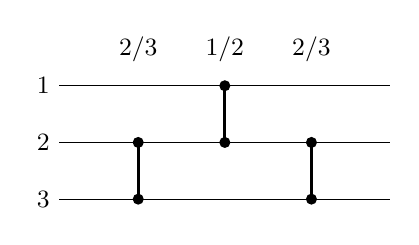
\begin{tikzpicture}[x=1cm,y=0.72cm,every node/.style={font=\small}]
  \foreach \y/\lab in {3/1,2/2,1/3} {
    \draw (0,\y) -- (4.2,\y);
    \node[left] at (0,\y) {\(\lab\)};
  }
  \draw[very thick] (1.0,2) -- (1.0,1);
  \fill (1.0,2) circle (2pt);
  \fill (1.0,1) circle (2pt);
  \node[above] at (1.0,3.25) {\(2/3\)};

  \draw[very thick] (2.1,3) -- (2.1,2);
  \fill (2.1,3) circle (2pt);
  \fill (2.1,2) circle (2pt);
  \node[above] at (2.1,3.25) {\(1/2\)};

  \draw[very thick] (3.2,2) -- (3.2,1);
  \fill (3.2,2) circle (2pt);
  \fill (3.2,1) circle (2pt);
  \node[above] at (3.2,3.25) {\(2/3\)};
\end{tikzpicture}

\smallskip
\textit{Mạng sắp xếp ba dây dùng trong phân tích bất đẳng thức.}
\end{center}

\[
\begin{array}{c|c|l}
\text{Giai đoạn} & \text{Sắp lại} & \text{Hệ bất đẳng thức}\\
\hline
1 & 2/3 &
A_{1,2}\ge A_{1,3};\ A_{1,1}\text{ với }A_{1,2}\text{ và }A_{1,3}\text{ chưa xác định}\\
2 & 1/2 &
A_{2,1}\ge A_{2,2};\ A_{2,1}\ge A_{2,3};\ A_{2,2}\text{ với }A_{2,3}\text{ chưa xác định}\\
3 & 2/3 &
A_{2,2}\ge A_{2,3};\ A_{2,1}\ge A_{2,2};\ A_{2,1}\ge A_{2,3}.
\end{array}
\]

Ta phát hiện rằng hệ bất đẳng thức của giai đoạn \(i\) có thể được suy ra từ
hệ bất đẳng thức của giai đoạn \(i-1\), căn cứ vào phép sắp lại được thực
hiện ở giai đoạn đó. Sau khi các dây đánh số \(i\) và \(j\) được sắp lại,
giữa hai dây \(i,j\) thiết lập một quan hệ bất đẳng thức, còn mọi bất đẳng
thức khác liên quan đến dây \(i\) và \(j\) đều cần được điều chỉnh. Suy diễn
giữa các bất đẳng thức thuộc về suy diễn logic. Chương trình của ta có thể
thực hiện loại suy diễn logic ấy không? Câu trả lời là có.

Giả sử ta đã có hệ bất đẳng thức ứng với giai đoạn \(i-1\). Giai đoạn \(i\)
sắp lại hai dây \(a,b\), với \(a<b\). Trước hết có \(A_{i,a}\ge A_{i,b}\).
Sau đó ta điều chỉnh mọi bất đẳng thức liên quan đến dây \(a,b\). Với \(a\)
và \(b\), xét riêng năm trường hợp.

\paragraph{Một, điều chỉnh mọi bất đẳng thức liên quan đến \(a\).}
\begin{enumerate}
  \item Nếu đã có \(A_{i-1,c}\ge A_{i-1,a}\), với \(c<a\) và \(c\ne b\), còn
  quan hệ giữa \(A_{i-1,c}\) và \(A_{i-1,b}\) chưa xác định, thì
  \(A_{i,a}\ge A_{i,b}\), \(A_{i,c}\ge A_{i,b}\), còn quan hệ giữa
  \(A_{i,c}\) và \(A_{i,a}\) chưa xác định.
  \item Nếu đã có \(A_{i-1,a}\ge A_{i-1,c}\), với \(a>c\) và \(c\ne b\), còn
  quan hệ giữa \(A_{i-1,c}\) và \(A_{i-1,b}\) chưa xác định, thì
  \(A_{i,a}\ge A_{i,b}\), \(A_{i,a}\ge A_{i,c}\), còn quan hệ giữa
  \(A_{i,b}\) và \(A_{i,c}\) chưa xác định.
  \item Nếu đã có \(A_{i-1,a}\ge A_{i-1,c}\) và
  \(A_{i-1,b}\ge A_{i-1,c}\), thì \(A_{i,a}\ge A_{i,b}\),
  \(A_{i,a}\ge A_{i,c}\), \(A_{i,b}\ge A_{i,c}\).
  \item Nếu đã có \(A_{i-1,a}\le A_{i-1,c}\) và
  \(A_{i-1,b}\le A_{i-1,c}\), thì \(A_{i,a}\ge A_{i,b}\),
  \(A_{i,a}\le A_{i,c}\), \(A_{i,b}\le A_{i,c}\).
  \item Nếu đã có \(A_{i-1,a}\ge A_{i-1,b}\), giữ nguyên.
\end{enumerate}

\paragraph{Hai, điều chỉnh mọi bất đẳng thức liên quan đến \(b\).}
\begin{enumerate}
  \item Nếu đã có \(A_{i-1,c}\ge A_{i-1,b}\), với \(c<b\) và \(c\ne a\), còn
  quan hệ giữa \(A_{i-1,c}\) và \(A_{i-1,a}\) chưa xác định, thì
  \(A_{i,a}\ge A_{i,b}\), \(A_{i,c}\ge A_{i,b}\), còn quan hệ giữa
  \(A_{i,c}\) và \(A_{i,a}\) chưa xác định.
  \item Nếu đã có \(A_{i-1,b}\ge A_{i-1,c}\), với \(b>c\) và \(c\ne a\), còn
  quan hệ giữa \(A_{i-1,c}\) và \(A_{i-1,a}\) chưa xác định, thì
  \(A_{i,a}\ge A_{i,b}\), \(A_{i,a}\ge A_{i,c}\), còn quan hệ giữa
  \(A_{i,b}\) và \(A_{i,c}\) chưa xác định.
  \item Nếu đã có \(A_{i-1,a}\ge A_{i-1,c}\) và
  \(A_{i-1,b}\ge A_{i-1,c}\), thì \(A_{i,a}\ge A_{i,b}\),
  \(A_{i,a}\ge A_{i,c}\), \(A_{i,b}\ge A_{i,c}\).
  \item Nếu đã có \(A_{i-1,a}\le A_{i-1,c}\) và
  \(A_{i-1,b}\le A_{i-1,c}\), thì \(A_{i,a}\ge A_{i,b}\),
  \(A_{i,a}\le A_{i,c}\), \(A_{i,b}\le A_{i,c}\), và
  \(A_{i-1,a}\ge A_{i-1,b}\).
  \item Nếu đã có \(A_{i-1,a}\ge A_{i-1,b}\), giữ nguyên.
\end{enumerate}

Phần thảo luận trên bao phủ mọi khả năng; khi lập trình cụ thể còn có thể
đơn giản hóa. Nếu suy diễn trên là đúng, thì hệ bất đẳng thức cuối cùng ta
thu được tương đương với hệ bất đẳng thức vốn ứng với mạng sắp xếp. Vì vậy ta
có thể phân tích quan hệ topo của hệ bất đẳng thức để chứng minh mạng sắp xếp
có thỏa yêu cầu hay không.

Dưới đây chứng minh suy diễn trên.

Muốn chứng minh suy diễn đúng, chỉ cần chứng minh từng trường hợp. Xét trường
hợp thứ nhất trong các bất đẳng thức liên quan đến \(a\), trừu tượng hóa
thành: ban đầu có ba số \(a,b,c\), với \(c\ge a\), còn quan hệ giữa \(c\) và
\(b\) chưa xác định; đặt \(a'=\max\{a,b\}\), \(b'=\min\{a,b\}\), \(c'=c\).
Cần chứng minh \(a'\ge b'\), \(c'\ge b'\), còn quan hệ giữa \(a'\) và \(c'\)
chưa xác định.

Chứng minh: nếu \(a\ge b\), do \(c\ge a\) nên \(c\ge a\ge b\). Khi đó
\(a'=a\), \(b'=b\), \(c'=c\), suy ra \(c'\ge a'\ge b'\). Nếu \(a<b\), ta có
\(c\ge a\), \(b>a\), còn quan hệ giữa \(b\) và \(c\) chưa xác định. Khi đó
\(a'=b\), \(b'=a\), \(c'=c\), nên \(c'\ge b'\), \(a'\ge b'\), còn quan hệ
giữa \(a'\) và \(c'\) chưa xác định. Tổng hợp lại, trong mọi trường hợp đều
có \(a'\ge b'\), \(c'\ge b'\), còn quan hệ giữa \(a'\) và \(c'\) có lúc chưa
xác định; tức quan hệ giữa \(a'\) và \(c'\) chưa xác định. Điều phải chứng
minh đã xong.

Các trường hợp khác cũng có thể chứng minh theo cách này. Do giới hạn dung
lượng, không trình bày chi tiết.

Từ đó thấy được tính đúng đắn của suy diễn. Vì vậy chỉ cần dựa trên các bất
đẳng thức đã thu được để kiểm tra xem hai dây bất kỳ có thứ tự topo hay
không, ta có thể chứng minh mạng sắp xếp có phải mạng sắp xếp hoàn chỉnh hay
không.

Ý nghĩa của việc giải bài này là nó chứng minh một điều: thiết kế chương
trình cũng có thể thực hiện một số suy diễn logic ``phức tạp''. Tuy nhiên,
giải bất đẳng thức đòi hỏi thí sinh phân tích vấn đề thật chi tiết, phân biệt
các tình huống, rồi thiết kế thuật toán.

\subsubsection{So sánh việc dùng bất đẳng thức với chiến lược thông thường}

Kết hợp giải bất đẳng thức với thiết kế chương trình tự thân đã là việc rất
có ý nghĩa: làm cho máy tính có một mức năng lực suy diễn logic nhất định,
qua đó bù đắp chỗ thiếu của máy tính.

Về hiệu suất, giải bất đẳng thức có hiệu suất cao vì nó dùng hệ bất đẳng thức
để thay cái cụ thể bằng cái trừu tượng, tiết kiệm chi phí liệt kê mọi tình
huống. Giải bất đẳng thức phù hợp với đặc điểm tốc độ tính toán của con người
``không nhanh''. Nếu máy tính vận dụng được nó, hiệu suất dĩ nhiên rất đáng
kể.

Thuật toán ``chuẩn'' cho Ví dụ 4 là dùng lý thuyết 0--1, xem
Phụ lục~\ref{app:notes}. Trên máy Pentium II 350, ta so sánh cách ấy với cách
giải bằng bất đẳng thức:
\[
\begin{array}{c|c|l}
\text{Cách giải} & \text{Độ phức tạp} & \text{Hiệu suất}\\
\hline
\text{Lý thuyết 0--1} & O(m\cdot 2^n) &
\text{khi }n\text{ hơn 20, thời gian đã không chịu nổi}\\
\text{Bất đẳng thức} & O(m\cdot n) &
\text{trong phạm vi bộ nhớ cho phép, thời gian luôn dưới }0.1\text{s}.
\end{array}
\]

Thực tế chứng minh rằng bất đẳng thức là một phương tiện giải bài cực kỳ tốt;
khi có thể, nên ưu tiên xét đến nó. Mấu chốt vẫn là sự vận dụng linh hoạt của
thí sinh.

Giống như phương trình, bất đẳng thức không bị giới hạn bởi ``bài toán
nguyên'' về phạm vi áp dụng; đây cũng là một ưu điểm của bất đẳng thức.

Dù vậy, cuối cùng bất đẳng thức vẫn có phạm vi áp dụng nhất định; trong nhiều
trường hợp hơn, cần phân tích cụ thể từng vấn đề cụ thể.

\subsection{Một loại bài đặc biệt: phương pháp xây dựng}

\begin{center}
\textit{Đi đến tận cùng của trí tưởng tượng}
\end{center}

Dùng phương pháp xây dựng để giải bài trước hết cần hiểu đề bài rất sâu, sau
đó còn phải có ý tưởng khéo léo. Nếu một vấn đề được giải bằng phương pháp
xây dựng, thì cả tư duy lẫn chương trình đều đã được tinh giản đến cực hạn.
Vì vậy có thể nói phương pháp xây dựng là thuật toán cấp cao nhất.

\subsubsection{Ứng dụng của phương pháp xây dựng}

Phương pháp xây dựng khác với bất đẳng thức và phương trình. Nó luôn là một
đối một: một vấn đề cụ thể ứng với một thuật toán cụ thể; giữa các vấn đề
khác nhau hiếm khi có liên hệ. Vì vậy phương pháp xây dựng không có khuôn mẫu
cố định để theo.

Chính vì tính chất đặc biệt ấy, liệt kê quá nhiều bài không có nhiều ý nghĩa.
Ở đây ta chỉ phân tích một bài kinh điển, coi như gợi mở.

\paragraph{Ví dụ 5. Trò chơi lấy số.}
\(N\) số nguyên dương được xếp thành một hàng ngang. Hai người luân phiên lấy
số; mỗi lần chỉ được lấy số ở đầu trái hoặc đầu phải, và giá trị số lấy được
là điểm của người đó trong lượt ấy. Khi mọi số đã bị lấy hết, tổng điểm mỗi
người nhận được là điểm cuối cùng của người đó; người có điểm cuối cùng lớn
hơn thắng. Nếu hai người bằng điểm, quy định người lấy trước thắng. Xem
Phụ lục~\ref{app:notes}.

Nếu khi trò chơi bắt đầu \(N\) là số chẵn, thì đối với người lấy trước tồn
tại một chiến lược chắc thắng. Hãy viết một chương trình, đóng vai người lấy
trước, tìm một chiến lược chắc thắng để chơi trò này với máy tính.

Ta có thể xử lý đề bài một chút: tô các đối tượng cần xử lý bằng các màu khác
nhau để phân biệt chúng, nhờ vậy mới thấy được một số bản chất ẩn. Tô các số
cần lấy bằng hai màu xen kẽ; ví dụ dưới đây là dãy
\[
\begin{array}{cccccc}
4&7&2&9&5&6\\
\text{đậm}&\text{nhạt}&\text{đậm}&\text{nhạt}&\text{đậm}&\text{nhạt}.
\end{array}
\]

Thực ra, người lấy trước có quyền lấy toàn bộ các số có màu mình muốn. Nói
cách khác, nếu người lấy trước muốn lấy ba số màu đậm \(4,2,5\), thì có thể
lấy được. Cụ thể như sau:
\begin{enumerate}
  \item Lấy 4; đối thủ chỉ có thể lấy 7 hoặc 6, mà chúng đều là màu nhạt.
  \item Dù đối thủ lấy thế nào, vẫn còn một và chỉ một số màu đậm có thể lấy;
  vậy lấy số đó.
  \item Đối thủ vẫn chỉ có thể chọn số màu nhạt.
  \item Tiếp tục như vậy.
\end{enumerate}

Cứ lấy như vậy, chỉ cần người đi trước mỗi lần đều chọn số màu đậm, nhất định
có thể lấy hết mọi số màu đậm.

Điều đó có nghĩa gì? Nghĩa là người đi trước chỉ cần chọn nhóm số có tổng lớn
hơn trong hai màu là có thể bảo đảm chiến thắng.

Vận dụng phương pháp xây dựng trong thi thật sự đòi hỏi sức sáng tạo của thí
sinh. Dĩ nhiên, cách giải của một bài toán rất đa dạng, đúng như câu mọi con
đường đều dẫn tới La Mã. Lời giải bằng phương pháp xây dựng có tính toán học
rất mạnh, đòi hỏi thí sinh có nền tảng toán tương đối sâu, đồng thời càng cần
năng lực quan sát nhạy bén và năng lực quy nạp, phỏng đoán.

\subsubsection{So sánh phương pháp xây dựng với các chiến lược khác}

Trước hết cần phân biệt phương pháp xây dựng với chiến lược tham lam, vốn rất
dễ bị nhầm lẫn. Thực ra khác biệt giữa phương pháp xây dựng và chiến lược
tham lam cũng rất rõ. Về bản chất, phương pháp xây dựng là thuật toán tìm lời
giải tối ưu, còn chiến lược tham lam là thuật toán tìm lời giải gần đúng.
Chiến lược tham lam xét vấn đề từ cục bộ rồi đưa ra lựa chọn; phương pháp xây
dựng thông qua phân tích toàn cục để xây dựng một chiến lược tối ưu có thể
chứng minh.

Về hiệu suất, phương pháp xây dựng là tối ưu trong mọi thuật toán; ngay cả
bất đẳng thức, phương trình trong chiến lược toán học, cũng như quy hoạch
động mà ta yêu thích, đều không sánh bằng.

Về phạm vi giải bài, phương pháp xây dựng được dùng rất rộng, nhưng nó lại
không có chút khả năng mở rộng nào đáng nói.

Là một phần của chiến lược toán học, dù có nhiều nhược điểm, phương pháp xây
dựng có hiệu suất rất hấp dẫn, trở thành mục tiêu theo đuổi của nhiều thí
sinh. Khi giải bài, nếu nghĩ ra thuật toán xây dựng, thuật toán ấy đương
nhiên là lựa chọn đầu tiên.

\section{Vì sao dùng chiến lược toán học}

\begin{center}
\textit{Tổng kết ứng dụng của chiến lược toán học}
\end{center}

Ở trên đã trình bày cụ thể ứng dụng của chiến lược toán học. Sau đây giải
thích vì sao cần dùng chiến lược toán học trong thi tin học. Có thể trả lời
câu hỏi này từ hai mặt.

\paragraph{Một, chiến lược toán học có thể giải các điểm khó của loại bài
này.}
Trước hết, chiến lược toán học có thể vượt qua ranh giới của bài toán nguyên,
mở rộng phạm vi giải bài, từ đó giải nhiều vấn đề mà chiến lược thông thường
không giải được. Thứ hai, chiến lược toán học có hiệu suất rất cao, mà hiệu
suất chính là điều ta mong muốn.

\paragraph{Hai, chiến lược toán học tránh được khuyết điểm chính của chiến
lược liệt kê.}
Chiến lược toán học và chiến lược liệt kê đứng ở hai độ cao khác nhau để nhìn
vấn đề. Vì sao nói như vậy?

Giả sử ta lần lượt dùng chiến lược toán học và chiến lược liệt kê để xử lý
cùng một vấn đề. Chiến lược toán học trước hết trừu tượng hóa vấn đề, lập ra
bất đẳng thức hoặc hệ phương trình, rồi dùng công cụ toán học tìm quan hệ phổ
quát tồn tại trong vấn đề. Phương pháp liệt kê thì ngược lại: trước hết phân
tích mọi trường hợp của vấn đề, rồi từ đó rút ra điểm chung và tổng kết quan
hệ phổ quát của vấn đề. Ta dùng chiến lược toán học chính là để bù đắp chi
phí quá lớn mà chiến lược liệt kê phải bỏ ra trong quá trình liệt kê mọi
trường hợp.

Chính vì chiến lược toán học và chiến lược liệt kê bổ sung cho nhau, nên
chiến lược toán học thường được dùng để xử lý những việc chiến lược liệt kê
không đảm đương nổi.

\paragraph{Lời bạt.}
Chiến lược toán học là kết tinh trí tuệ của con người; vận dụng tốt chiến
lược toán học là yêu cầu cơ bản đối với thí sinh. Chiến lược toán học có ưu
điểm, cũng có nhược điểm. Thực ra, quy mô vấn đề mà mỗi chiến lược có thể xử
lý đều hữu hạn. Khi lập trình giải quyết, phải xác định rõ quy mô vấn đề, từ
đó mưu hoạch chiến lược thích hợp và xây dựng thuật toán tương ứng. Chiến
lược toán học có hiệu suất cao vì nó có tính nhắm đích cao hơn chiến lược
liệt kê thông thường. Nói chung, thuật toán càng nhắm đích cao thì hiệu suất
càng cao, như phương pháp xây dựng; khả năng mở rộng càng thấp, và việc xây
dựng cũng càng khó. Với mọi chiến lược, ta có thể tổng kết rằng khả năng mở
rộng và hiệu suất, cũng như độ dễ xây dựng và hiệu suất, về cơ bản đều có
quan hệ tỉ lệ nghịch. Giải quyết vấn đề chính là chọn ra một điểm cân bằng
tốt nhất trong đó.

Trong ``bảng cách giải bài'' của nhà toán học Polya từng có câu: ``Nếu bạn
không thể giải được bài toán này, bạn có thể giải một phần của bài toán hay
không?'' Khi gặp một bài toán lạ, ta nên thử chiến lược toán học trước. Ngay
cả khi chiến lược toán học không thể giải hoàn toàn bài toán, ta vẫn có thể
đơn giản hóa một phần, từ đó trải đường cho việc chọn chiến lược khác lần
nữa, như Ví dụ 1. Chính vì ưu thế của chiến lược toán học, ta nói rằng thử
chiến lược toán học vốn nên là bước đầu tiên khi xử lý vấn đề.

Toán học không chỉ là nền tảng của chiến lược toán học, mà còn là nền tảng
của toàn bộ tin học. Hiện nay đề thi tin học ngày càng phức tạp; thời đại chỉ
máy móc áp dụng thuật toán đã qua. Hiện tại, đề thi kiểm tra nhiều hơn sự
phối hợp giữa các thuật toán. Toán học là một phần không thể tách rời của thi
tin học, và liên hệ giữa toán học với đề bài cũng ngày càng chặt chẽ; việc
kết hợp ứng dụng toán học với giải bài tin học e rằng cũng là một xu hướng.

Toán học là một vẻ đẹp. Có một nhà khoa học từng nói: nếu phải chọn giữa chân
lý và cái đẹp, tôi sẵn lòng chọn cái đẹp. Dĩ nhiên, trong rất nhiều vấn đề,
chân lý và cái đẹp là thống nhất, nhất là trong một ngành như toán học. Trong
lập trình, nếu có thể hiểu, nắm vững và ứng dụng toán học tốt hơn, nhất định
ta sẽ đạt đến sự thống nhất hài hòa giữa chân lý và cái đẹp.

Xin lấy điều đó làm kết thúc cho bài viết này.

\appendix
\section{Phụ lục}
\label{app:notes}

\begin{enumerate}
  \item Chiến lược toán học nói ở đây cũng thuộc phạm vi trí tuệ nhân tạo,
  cụ thể là hệ chuyên gia trong trí tuệ nhân tạo. Nói ngắn gọn, hệ chuyên gia
  là làm cho máy tính mô phỏng nhiều nhất có thể quá trình ra quyết định và
  làm việc của chuyên gia con người khi giải một số vấn đề thực tế; tức mô
  phỏng phương pháp, kỹ xảo và bước đi mà chuyên gia con người dùng tri thức
  và kinh nghiệm của họ để giải quyết vấn đề trước mắt. Ở đây, ta đưa kỹ xảo
  giải bài của mình vào lập trình.

  \item ``Bài toán quân bài'' lấy từ bài 2 ngày thi thứ hai của IOI 1999. Đề
  gốc xem trong \textit{Olympiad Tin học}, số 4 năm 1999. Nhập và xuất giống
  đề gốc.

  \item ``Bài toán điện trở'' lấy từ chuyên mục thi đài do thầy Wu Wenhu và
  các thầy khác phụ trách, trong \textit{Computer Enthusiast}, số 12 năm
  1999.

  \item ``Đèn tháp tam giác'' lấy từ bài 2 của NOI 1996. Cách giải bằng
  phương trình của bài này được mô tả ngắn gọn như sau: trạng thái của một
  bóng đèn bất kỳ đều có thể suy ra từ trạng thái của hai bóng đèn phía dưới
  nó. Vì vậy, với một bóng đèn \(b_{ij}\) đã biết trạng thái, tức bóng thứ
  \(j\) ở hàng thứ \(i\), lấy bóng này làm đỉnh, kéo hai cạnh xuống dưới, và
  cùng đáy \(x_j,\ldots,x_{N+j-i}\) tạo thành một tam giác có \(N+1-i\) hàng.
  Trạng thái của \(b_{ij}\) có thể suy ra từ
  \(x_j,\ldots,x_{N+j-i}\), nên có thể lập một phương trình. Nếu có \(p\) bóng
  đã biết, ta có \(p\) phương trình tuyến tính. Giải hệ bất định này là giải
  được bài.

  \item ``Phương án phân tích tối ưu'' lấy từ kỳ tuyển chọn đội Trung Quốc
  dự IOI 1996. Nhập và xuất giống đề gốc.

  \item ``Bài toán mạng sắp xếp'' lấy từ đề huấn luyện đội tuyển Bắc Kinh cho
  NOI 1999.

  \item Lý thuyết 0--1 là một phương pháp giải bài toán mạng sắp xếp. Nói
  ngắn gọn, trong sắp xếp chỉ có ba quan hệ lớn nhỏ: lớn hơn, nhỏ hơn hoặc
  bằng. Vì vậy, để kiểm tra một mạng sắp xếp \(n\) hàng có phải mạng sắp xếp
  hoàn chỉnh hay không, ta có thể kiểm tra mọi dãy \(n\) bit tạo bởi 0 và 1;
  hai việc này hoàn toàn tương đương.

  \item ``Trò chơi lấy số'' lấy từ một bài của IOI 1996. Nhập và xuất giống
  đề gốc.

  \item ``Bài toán hệ số truy hồi của hàm lũy thừa'' trong kỳ tuyển chọn tỉnh
  Phúc Kiến cho NOI 1999 là một bài phương pháp xây dựng rất hay. Vì
  \textit{Olympiad Tin học}, số 3 năm 1999, đã có cách giải và chứng minh
  rất chi tiết, ở đây không trình bày thêm.
\end{enumerate}

\section{Tài liệu tham khảo}

\begin{enumerate}
  \item \textit{Olympiad Tin học}, tập 1 và tập 2.
  \item \textit{Tuyển tập luận văn xuất sắc đội tuyển tập huấn Trung Quốc
  IOI 1998}.
  \item Wu Wenhu, Wang Jiande, \textit{Hướng dẫn thi Olympic tin học quốc tế
  và trong nước cho thanh thiếu niên}, Nhà xuất bản Đại học Thanh Hoa, 1997.
  \item Wu Wenhu, Wang Jiande, \textit{Phân tích đề thi Olympic tin học quốc
  tế và trong nước năm 1996}, Nhà xuất bản Đại học Thanh Hoa, 1997.
  \item Lu Kaicheng, Lu Kaiming, \textit{Lý thuyết đồ thị và ứng dụng}, Nhà
  xuất bản Đại học Thanh Hoa, 1995, bản thứ hai.
  \item Cai Zixing, Xu Guangyou, \textit{Trí tuệ nhân tạo và ứng dụng}, Nhà
  xuất bản Đại học Thanh Hoa, 1996, bản thứ hai.
  \item Tan Haoqiang, \textit{Ngôn ngữ BASIC: thiết kế chương trình có cấu
  trúc}, Nhà xuất bản Khoa học Kỹ thuật Trung Quốc, 1990.
\end{enumerate}

\section{Mã nguồn}

\subsection{Mã nguồn của Ví dụ 1}

\begingroup
\scriptsize
\begin{verbatim}
{$A+,B-,D+,E+,F-,G-,I+,L+,N-,O-,P-,Q-,R-,S+,T-,V+,X+}
{$M 65520,0,655360}
Program Flat;
Type Array_type=array[1..200] of longint; {kieu mang}
    Way_typep=array[1..10000] of integer;
    Way_type=array[1..2] of ^Way_typep; {kieu mang phuong an di chuyen}
Var Poles, {trang thai cac cot bai}
   Answers:Array_type; {nghiem cua phuong trinh, tong so bai moi cot can chuyen}
   FinalWay:Way_type; {phuong an di chuyen tot nhat}
   N:integer; {so cot}
   FinalWaynum, {so buoc cua phuong an tot nhat}
   Average:longint; {so bai trung binh moi cot}
   time:longint; {thoi gian}
Procedure Init; {khoi tao}
var Total:longint; {tong so bai}
   i:integer;
   filename:string; {ten tep vao}
   f:text; {tep}
Begin {Init}
 time:=meml[$40:$6c];
 filename:='Flat.inp';
 assign(f,filename);
 reset(f);
 read(f,N);
 Total:=0;
 for i:=1 to N do
   begin
     read(f,Poles[i]);
     Total:=Total+Poles[i]; {tong so bai}
   end;
 Average:=Total div N; {trang thai cuoi: so bai moi cot}
 close(f);
End; {Init}

Procedure Compute; {giai phuong trinh}
var Equations:Array_type; {phuong trinh}
   min:longint; {nghiem nho nhat cua phuong trinh}
   i:integer;
Begin {Compute}
 Equations[1]:=Poles[1]-Average;
 for i:=2 to N-1 do
   Equations[i]:=Poles[i]-Average;
 for i:=2 to N-1 do
   Equations[i]:=Equations[i]+Equations[i-1];
 Answers[1]:=0;
 for i:=2 to N do
   Answers[i]:=(Equations[i-1]-Answers[i-1])*(-1);
 min:=Answers[1];
 for i:=2 to N do
   if min>Answers[i] then min:=Answers[i];
 for i:=1 to N do
   Answers[i]:=Answers[i]-min;
End; {Compute}

Procedure Find;
Var Move, {trang thai cac cot bai}
  Answers_Find:Array_type; {tong so bai moi cot con can chuyen}
  Choice:array[1..200,1..2] of Longint; {so bai moi cot co the chuyen}
  Way:Way_type; {phuong an di chuyen}
  Waynum, {so lan di chuyen}
  Agreenum, {so bai duoc phep chuyen}
  Movenum, {tong so bai con phai chuyen}
  Change:longint; {bien tam de hoan doi}
  i,j,k:integer;
Begin {Find}
 randomize;
 FinalWaynum:=1000000000;
 new(FinalWay[1]); new(FinalWay[2]);
 new(Way[1]); new(Way[2]);
 repeat {repeat}
  Movenum:=0;
  for i:=1 to N do
    Movenum:=Movenum+Answers[i];
  Move:=Poles; Answers_Find:=Answers;
  Waynum:=0;
  repeat {tinh so bai moi cot co the chuyen}
    if Move[1]>=Answers_Find[1] then Choice[1,1]:=Answers_Find[1]
                         else Choice[1,1]:=Move[1];
    if Move[N]>=Answers_Find[N] then Choice[N,1]:=Answers_Find[N]
                         else Choice[N,1]:=Move[N];
    for i:=2 to N-1 do
      begin
        if Move[i]>=(Answers_Find[i] shl 1) then Choice[i,1]:=Answers_Find[i]
                                else Choice[i,1]:=Move[i] shr 1;
        Choice[i,2]:=i;
      end;
    Choice[1,2]:=1; Choice[N,2]:=N;
    for i:=1 to 3 do {tim ba cot co the chuyen nhieu bai nhat}
      begin
        k:=i;
        for j:=i+1 to N do
          if Choice[k,1]<Choice[j,1] then k:=j;
        Change:=Choice[k,1]; Choice[k,1]:=Choice[i,1]; Choice[i,1]:=Change;
        Change:=Choice[k,2]; Choice[k,2]:=Choice[i,2]; Choice[i,2]:=Change;
      end;
    k:=random(3)+1; {chon ngau nhien mot trong ba cot nhieu nhat}
    {di chuyen cang nhieu bai cua cot nay cang tot}
    if (Choice[k,2]>1) and (Choice[k,2]<N) then
      begin
        Agreenum:=Answers_Find[Choice[k,2]];
        if (Agreenum*2)>Move[Choice[k,2]] then
          Agreenum:=Move[Choice[k,2]] div 2;
        Move[Choice[k,2]]:=Move[Choice[k,2]]-Agreenum*2;
        Move[Choice[k,2]+1]:=Move[Choice[k,2]+1]+Agreenum;
        Move[Choice[k,2]-1]:=Move[Choice[k,2]-1]+Agreenum;
        Answers_Find[Choice[k,2]]:=Answers_Find[Choice[k,2]]-Agreenum;
        Movenum:=Movenum-Agreenum;
      end;
    if (Choice[k,2]=1) or (Choice[k,2]=N) then
      begin
       Agreenum:=Answers_Find[Choice[k,2]];
       if Agreenum>Move[Choice[k,2]] then Agreenum:=Move[Choice[k,2]];
       Move[Choice[k,2]]:=Move[Choice[k,2]]-Agreenum;
       if Choice[k,2]=1 then
         Move[Choice[k,2]+1]:=Move[Choice[k,2]+1]+Agreenum
                  Else
         Move[Choice[k,2]-1]:=Move[Choice[k,2]-1]+Agreenum;
       Answers_Find[Choice[k,2]]:=Answers_Find[Choice[k,2]]-Agreenum;
       Movenum:=Movenum-Agreenum;
     end;
     if Agreenum>0 then
       begin
         inc(Waynum);
         Way[1]^[Waynum]:=Choice[k,2];
         Way[2]^[Waynum]:=Agreenum;
       end;
  until Movenum=0; {tong so bai con phai chuyen bang 0, da chuyen xong}
  if Waynum<FinalWaynum then begin FinalWaynum:=Waynum; FinalWay:=Way; end;
  {neu tim duoc phuong an tot hon thi ghi lai}
 until ((meml[$40:$6c]-time)/18.2)>2; {lap den khi het thoi gian cho phep}
End; {Find}

Procedure Print; {xuat}
var i:integer;
   filename:string; {ten tep ra}
   f:text; {tep}
Begin {Print}
 filename:='flat.out';
 assign(f,filename);
 rewrite(f);
 writeln(f,FinalWaynum); {xuat tong so lan di chuyen}
 for i:=1 to FinalWaynum do {lan luot xuat cach di chuyen}
   writeln(f,FinalWay[1]^[i]:3,' ',FinalWay[2]^[i]:4);
 close(f);
End; {Print}

BEGIN {main}
 Init;
 Compute;
 Find;
 Print;
END. {main}
\end{verbatim}
\endgroup

\subsection{Mã nguồn của Ví dụ 2}

\begingroup
\scriptsize
\begin{verbatim}
{$A+,B-,D+,E+,F-,G-,I+,L+,N-,O-,P-,Q-,R-,S+,T-,V+,X+}
{$M 65520,0,655360}
PROGRAM Uncoil_Resistance;
Type array_type=array[0..100] of real;
Var Resistance:array[0..100] of ^array_type; {tat ca dien tro}
  Equations:array[0..100] of ^array_type; {he phuong trinh}
  Num:array[1..100,1..100] of byte; {so hieu dien tro}
  Line:array[1..100,1..2] of byte; {dien tro ung voi moi so hieu}
  Direct:array[1..100] of shortint; {huong duong di}
  Mark:array[1..100] of shortint; {danh dau thu tu nut tren duong di}
  Connects:array[1..100,1..100] of shortint; {tinh lien thong}
  Points:set of 1..100; {cac diem tren duong di}
  Lines:set of 1..100; {cac dien tro tren duong di}
  N,
  M,
  l,
  a,b:integer;
  R:real; {tong dien tro}

Procedure Init; {doc thong tin dien tro va khoi tao}
var filename:string;
   f:text;
   i,j,k,
   p,q:integer;
   js:integer;
Begin {Init}
 filename:='Input.txt';
 assign(f,filename);
 reset(f);
 readln(f,N);
 readln(f,M);
 readln(f,a,b);
 for p:=1 to 100 do
   begin
     new(Resistance[p]);
     new(Equations[p]);
     for q:=0 to 100 do
       begin
         Resistance[p]^[q]:=0;
         Equations[p]^[q]:=0;
       end;
   end;
 js:=0;
 for p:=1 to M do
   begin
     readln(f,i,j,k);
     Line[p,1]:=i; Line[p,2]:=j;
     if Resistance[i]^[j]=0 then begin
                          Resistance[i]^[j]:=k;
                          Resistance[j]^[i]:=k;
                          Num[i,j]:=p; Num[j,i]:=p;
                         end
                      else begin {gop dien tro song song thuan}
                          Resistance[i]^[j]:=1/(1/Resistance[i]^[j]+1/k);
                          Resistance[j]^[i]:=Resistance[i]^[j];
                          Line[p,1]:=0; Line[p,2]:=0;
                          inc(js);
                         end;
   end;
 M:=M-js;
 close(f);
End; {Init}

Procedure Research_Circle; {tim vong}
var Way:array[1..100] of integer;
  Done,Wait:set of 1..100;
  escape:boolean;
  p,q,ll,i,j,k,x:integer;

Begin {Research_Circle}

 {xay dung duong di}
 for i:=1 to N do
   Way[i]:=-1;
 Way[a]:=0; Done:=[]; Wait:=[a];
 repeat
   k:=10000; j:=-1;
   for i:=1 to N do
     if (i in Wait) and (k>Way[i]) then begin k:=Way[i]; j:=i; end;
   Done:=Done+[j]; Wait:=Wait-[j];
   for i:=1 to N do
     if (Resistance[j]^[i]>0) and ((Way[i]>(Way[j]+1)) or (Way[i]=-1)) then
       begin
         Way[i]:=Way[j]+1;
         Wait:=Wait+[i];
       end;
 until Wait=[];
 {ghi cac diem tren duong di va huong duong di}
 for i:=1 to M do
   Direct[i]:=0;
 i:=b; Points:=[b]; Lines:=[];
 repeat
   for j:=1 to N do
     if Way[j]=(Way[i]-1) then begin k:=j; j:=N; end;
   Points:=Points+[k];
   if k<i then Direct[Num[k,i]]:=1
          else Direct[Num[k,i]]:=-1;
   Lines:=Lines+[Num[k,i]];
   i:=k;
 until i=a;
 {mo rong duong di}
 repeat
   escape:=true;
   for i:=1 to M do
     if Direct[i]<>0 then
       for j:=1 to N do
         if (Not (j in Points)) and
            (Resistance[Line[i,1]]^[j]>0) and
            (Resistance[Line[i,2]]^[j]>0) then
            begin
             escape:=false;
             Points:=Points+[j];
             Lines:=Lines+[Num[Line[i,1],j]];
             Lines:=Lines+[Num[Line[i,2],j]];
             Lines:=Lines-[Num[Line[i,1],Line[i,2]]];
             if Line[i,1]<j then Direct[Num[Line[i,1],j]]:=1
                         else Direct[Num[Line[i,1],j]]:=-1;
             if j<Line[i,2] then Direct[Num[Line[i,2],j]]:=1
                         else Direct[Num[Line[i,2],j]]:=-1;
             if (Line[i,1]<Line[i,2]) and (Direct[i]=-1) then
               begin
                 Direct[Num[Line[i,1],j]]:=-Direct[Num[Line[i,1],j]];
                 Direct[Num[Line[i,2],j]]:=-Direct[Num[Line[i,2],j]];
               end;
            end;
 until escape;
 {danh dau thu tu cac nut tren duong di}
 x:=1; Mark[a]:=x;
 q:=a; ll:=q;
 repeat
  for p:=1 to N do
    if (p<>q) and (Num[q,p] in Lines) and
       (((p<q) and (Direct[Num[q,p]]=-1)) or
        ((p>q) and (Direct[Num[q,p]]=1))) then
      begin ll:=p; p:=N; end;
  q:=ll;
  inc(x); Mark[q]:=x;
 until q=b;
End; {Research_Circle}

Procedure Connect; {tinh lien thong cua cac diem ngoai duong di}
var i,j,k:integer;
Begin {Connect}
 for i:=1 to N-1 do
   for j:=i+1 to N do
     if (i<>j) and (Resistance[i]^[j]>0) and (not (Num[i,j] in lines)) then
       begin Connects[i,j]:=1; Connects[j,i]:=1; end
       else begin Connects[i,j]:=-9; Connects[j,i]:=-9; end;
 for i:=1 to N do
   Connects[i,i]:=0;
 for k:=1 to N do
   if not (k in points) then
   for i:=1 to N do
     if (i<>k) and (Connects[i,k]>0) then
       for j:=1 to N do
         if (i<>j) and (j<>k) and (Connects[k,j]>0) and
            ((Connects[i,j]>(Connects[i,k]+Connects[k,j])) or
             (Connects[i,j]=-9)) then
           Connects[i,j]:=Connects[i,k]+Connects[k,j];
End; {Connect}

Procedure List; {lap phuong trinh}
var i,j,k,p,q,ll:integer;
    Ways:array[1..100] of byte;
    pd:boolean;
Begin {List}
  for i:=1 to N do {voi moi nut}
    begin
      for j:=1 to N do
         if (i<>j) and (Resistance[i]^[j]>0) then
           begin
             if i<j then Equations[i]^[Num[i,j]]:=1
                   else Equations[i]^[Num[i,j]]:=-1;
           end;
      if i=a then Equations[i]^[0]:=-1;
      if i=b then Equations[i]^[0]:=1;
    end;
  Research_Circle;
  Connect;
  l:=0;
  for i:=1 to N do {lap phuong trinh cho cac vong}
    for j:=1 to N do
        if (i<>j) and (i in Points) and (j in Points) and
           (Connects[i,j]>0) and (Mark[i]<Mark[j]) then
         begin
           k:=2; Ways[1]:=i; Ways[2]:=0;
           repeat {tim vong}
             pd:=false;
             for p:=Ways[k]+1 to N do
               if (Connects[Ways[k-1],j]=(Connects[p,j]+1)) and
                  (Resistance[Ways[k-1]]^[p]>0) then
                begin
                 Ways[k]:=p; Ways[k+1]:=0; k:=k+1; p:=N;
                 pd:=true;
                end;
             if not pd then k:=k-1;
             if Ways[k-1]=j then begin {tim thay vong}
                       l:=l+1; {them mot phuong trinh}
                       for p:=1 to k-2 do
                         begin
                           if Ways[p]>Ways[p+1] then
                             Equations[N+l]^[Num[Ways[p],Ways[p+1]]]:=1
                           else
                             Equations[N+l]^[Num[Ways[p],Ways[p+1]]]:=-1;
                         end;
                       q:=i; ll:=q;
                       repeat
                         for p:=1 to N do
                           if (p<>q) and (Num[q,p] in Lines) and
                              (((p<q) and (Direct[Num[q,p]]=-1)) or
                               ((p>q) and (Direct[Num[q,p]]=1))) then
                             begin ll:=p; p:=N; end;
                         Equations[N+l]^[Num[q,ll]]:=Direct[Num[q,ll]];
                         q:=ll;
                       until q=j;
                       for p:=1 to M do
                         if Equations[N+l]^[p]<>0 then
                            Equations[N+l]^[p]:=
                              Equations[N+l]^[p]*Resistance[Line[p,1]]^[Line[p,2]];
                      end;
         until k=1;
       end;
 inc(l);
 for p:=0 to M do
   Equations[N+l]^[p]:=0;
 j:=a; k:=j;
 repeat
   for p:=1 to N do
     if (p<>j) and (Num[j,p] in Lines) and
        (((p<j) and (Direct[Num[j,p]]=-1)) or
         ((p>j) and (Direct[Num[j,p]]=1))) then
   begin k:=p; p:=N; end;
   Equations[N+l]^[Num[j,k]]:=Direct[Num[j,k]];
   j:=k;
 until j=b;
 for p:=1 to M do
   if Equations[N+l]^[p]<>0 then
      Equations[N+l]^[p]:=
        Equations[N+l]^[p]*Resistance[Line[p,1]]^[Line[p,2]];
End; {List}

Procedure Uncoil; {dung khu Gauss de giai he phuong trinh}
Var Answers:array[0..100] of real; {nghiem cua he phuong trinh}
  i,j,k:integer;
  U:integer;
  Change:real;
  Compute:real;
Begin {Uncoil}
 for i:=1 to M+1 do
   begin
    if Equations[i]^[i-1]=0 then
      begin
        for j:=i+1 to N+l do
          if Equations[j]^[i-1]<>0 then begin k:=j; j:=N+l; end;
        for j:=i-1 to M do
          begin
            Change:=Equations[i]^[j];
            Equations[i]^[j]:=Equations[k]^[j];
            Equations[k]^[j]:=Change;
          end;
      end;
    for j:=i+1 to N+l do
      if Equations[j]^[i-1]<>0 then
        begin
          for k:=i to M do
            Equations[j]^[k]:=
              Equations[i]^[k]*Equations[j]^[i-1]/Equations[i]^[i-1]-
              Equations[j]^[k];
          Equations[j]^[i-1]:=0;
        end;
   end;
 U:=100; {thay vao de giai}
 Answers[M+1]:=U/Equations[M+1]^[M];
 for i:=M downto 1 do
   begin
    Compute:=0;
    for j:=M downto i do
      Compute:=Compute+Equations[i]^[j]*Answers[j+1];
    Answers[i]:=-Compute/Equations[i]^[i-1];
   end;
 R:=U/Answers[1]; {tinh tong dien tro}
End; {Uncoil}

Procedure Print; {xuat tong dien tro}
Begin {Print}
 writeln(abs(R):0:2);
End; {Print}

BEGIN {main}
 Init;
 List;
 Uncoil;
 Print;
END. {main}
\end{verbatim}
\endgroup

\subsection{Mã nguồn của Ví dụ 3}

\begingroup
\scriptsize
\begin{verbatim}
{$A+,B-,D+,E+,F-,G-,I+,L+,N-,O-,P-,Q-,R-,S+,T-,V+,X+}
{$M 65520,0,655360}
Program MaxMul;
Const Max=1000; {gia tri lon nhat cua N}
Type Multype=array[0..255] of integer; {kieu luu tich}
Var D:array[1..50] of integer; {luu cac so trong phan tich}
  i,j,n,m:integer;
  Mul:MulType; {tich}
  Change:Boolean;

Procedure Multhem(n:integer); {Mul=Mul*N}
Begin
 for i:=1 to Mul[0] do
   Mul[i]:=Mul[i]*n;
 for i:=1 to Mul[0] do
   begin
    Mul[i+1]:=Mul[i+1]+Mul[i] div 10;
    Mul[i]:=Mul[i] mod 10;
   end;
 i:=Mul[0]+1;
 While Mul[i]<>0 do
   begin
    inc(Mul[0]);
    Mul[i+1]:=Mul[i+1]+Mul[i] div 10;
    Mul[i]:=Mul[i] mod 10;
    inc(i);
   end;
End;

Procedure GetMul; {nhan cac so da phan tich va luu trong Mul}
Var i,j:byte;
Begin
 fillchar(Mul,sizeof(Mul),0);
 Mul[0]:=1;
 Mul[1]:=1;
 for i:=1 to m do
   Multhem(D[i]);
End;

BEGIN {main}
 repeat
   write('N=');
   readln(n);
   if (n>Max) or (n<3) then writeln('Out of Range!');
 until (n<=Max) and (n>=3);
 j:=2;
 m:=1;
 While (n>=2*j+1) do {tach n thanh cang nhieu so khac nhau >1 cang tot}
   begin
     D[m]:=j;
     n:=n-j;
     j:=j+1;
     m:=m+1;
   end;
 D[m]:=n;
 for i:=m-1 downto 1 do {dieu chinh de cac so cang sat nhau cang tot}
   if ((i=m-1) and (D[m]>D[m-1]+2)) or
      ((i<>m-1) and (D[m]>D[m-1]+1)) then
     begin
       dec(D[m]);
       inc(D[i]);
     end
     else Break;
 for i:=1 to m-1 do {xuat cac so}
   write(D[i],',');
 writeln(D[m]);
 GetMul; {tinh tich}
 For i:=Mul[0] downto 1 do {xuat tich}
  write(Mul[i]);
 writeln;
END. {main}
\end{verbatim}
\endgroup

\subsection{Mã nguồn của Ví dụ 4}

\begingroup
\scriptsize
\begin{verbatim}
{$A+,B-,D+,E+,F-,G-,I+,L+,N-,O-,P-,Q-,R-,S+,T-,V+,X+}
{$M 65520,0,655360}
Program Taxis_Net;
Var Inequality:array[1..100,1..100] of shortint; {luu he bat dang thuc}
   N,M:word; {N la so day dan; M la so cau}
Procedure Work;
Var p,
   a,b,c,
   Change:integer;
Begin {Work}
 assign(input,'Input.txt');
 reset(input);
 readln(N);
 readln(M);
 fillchar(Inequality,sizeof(Inequality),0);
 for p:=1 to M do {lan luot xu ly tung cau}
   begin
     readln(a,b);
     if a>b then begin
                   Change:=a;
                   a:=b;
                   b:=Change;
                 end;
     if Inequality[a,b]=0 then
       begin
         Inequality[a,b]:=1; Inequality[b,a]:=-1;
         for c:=1 to N do
           if (c<>a) and (c<>b) and (Inequality[a,c]<>0) then
                 {dieu chinh moi bat dang thuc lien quan den a}
             begin
               if (Inequality[c,a]=1) and (Inequality[c,b]=0) then
                 begin
                   Inequality[c,b]:=1; Inequality[b,c]:=-1;
                   Inequality[c,a]:=0; Inequality[a,c]:=0;
                 end;
               if (Inequality[c,a]=-1) and (Inequality[c,b]=0) then
                 begin
                   Inequality[c,a]:=-1; Inequality[a,c]:=1;
                   Inequality[c,b]:=0; Inequality[b,c]:=0;
                 end;
             end;
         for c:=1 to N do
           if (c<>a) and (c<>b) and (Inequality[c,b]<>0) then
                 {dieu chinh moi bat dang thuc lien quan den b}
             begin
               if (Inequality[c,b]=1) and (Inequality[c,a]=0) then
                 begin
                   Inequality[c,b]:=1; Inequality[b,c]:=-1;
                   Inequality[c,a]:=0; Inequality[a,c]:=0;
                 end;
               if (Inequality[c,b]=-1) and (Inequality[c,a]=0) then
            begin
               Inequality[a,c]:=1; Inequality[c,a]:=-1;
               Inequality[c,b]:=0; Inequality[b,c]:=0;
            end;
          end;
       end;
   end;
 close(input);
 assign(output,'Output.txt');
 rewrite(output);
 for p:=1 to N-1 do
   if Inequality[p,p+1]<>1 then begin {kiem tra mang sap xep co hop le khong}
                         writeln('No!'); {khong hop le}
                         close(output);
                         halt;
                       end;
 writeln('Yes!'); {hop le}
 close(output);
End; {Work}

BEGIN {main}
 Work;
END. {main}
\end{verbatim}
\endgroup

\subsection{Mã nguồn của Ví dụ 5}

\begingroup
\scriptsize
\begin{verbatim}
{$A+,B-,D+,E+,F-,G-,I+,L+,N-,O-,P-,Q-,R-,S+,T-,V+,X+}
{$M 65520,0,655360}
Program IOI96_Program3;
Uses Play;
Const Max=100; {gia tri lon nhat cua N}
Var n:byte;
  D:array[1..Max] of byte; {N so trong day}
  MyScore,YourScore,
  Start:integer;
  SelectOdd:boolean; {chon vi tri le hay vi tri chan}

Procedure Init; {doc tep va khoi tao}
Var i,j:integer;
   Odd,Even:integer; {Odd la tong vi tri le; Even la tong vi tri chan}
Begin
 assign(input,'Input.txt');
 reset(input);
 readln(n);
 for i:=1 to n do
   readln(D[i]);
 close(input);
 Odd:=0;
 Even:=0;
 for i:=1 to n div 2 do {tinh tong vi tri le va vi tri chan}
   begin
    Odd:=Odd+D[i*2-1];
    Even:=Even+D[i*2];
   end;
 if Odd>Even then begin {neu tong vi tri le lon hon}
               MyScore:=Odd; {chon lay tat ca so o vi tri le}
               YourScore:=Even;
               SelectOdd:=true;
            end
         else begin {nguoc lai}
             MyScore:=Even; {chon lay tat ca so o vi tri chan}
             YourScore:=Odd;
             SelectOdd:=false;
            end;
End;

Procedure Task;
Var i:integer;
   C:Char;
Begin
 StartGame;
 Start:=1;
 for i:=1 to n div 2 do
   begin
    if Odd(Start)=SelectOdd then begin
                         MyMove('L');
                         inc(Start);
                        end
                     else begin
                         MyMove('R');
                         YourMove(C);
                         if C='L' then inc(Start);
                        end;
   end;
 assign(output,'Output.txt');
 rewrite(output);
 writeln(MyScore,' ',YourScore);
 close(output);
End;

BEGIN {main}
 Init;
 Task;
END. {main}
\end{verbatim}
\endgroup

Đơn vị \texttt{PLAY} dùng để kiểm thử trong Ví dụ 5:

\begingroup
\scriptsize
\begin{verbatim}
UNIT PLAY;

INTERFACE
 PROCEDURE STARTGAME;
 PROCEDURE MYMOVE(C:CHAR);
 PROCEDURE YOURMOVE(VAR C:CHAR);

IMPLEMENTATION

PROCEDURE STARTGAME;
Begin

End;

PROCEDURE MYMOVE(C:CHAR);
Begin

End;

PROCEDURE YOURMOVE(VAR C:CHAR);
Begin
 C:='L';
End;

END.
\end{verbatim}
\endgroup

\end{document}
